\chapter{Path Planning}
\label{chapter:pathplanning}
In this chapter, the planning and deliberation of \textit{where to sense at the moment of opportunity} will be presented. The problem definition of any planning algorithm for adaptive sampling, once the robot is in the water, becomes "based on current observations and models, what should the robot do \textit{now}?" First, the simplest planning algorithms are presented, the subsumption based architectures, before more deliberative methods are presented. 

\section{Subsumption based}
Subsumption architectures \cite{fossum2019adaptive}, or ad hoc behaviors, are a set of behaviors defined by a \textit{Sense\textrightarrow Act} strategy, where the model is baked into the assumptions of the behavior. The behavior in such a method must be customized for the purpose, and is generally not equipped to handle unexpected events. Implementation of subsumption architectures are usually done as a finite state machine, such as is presented in \cite{fossum2021adaptive}. The "\textit{planning}" done in these architectures lies in the rule-based behavior, and depends on the internal state of the AUV. This does not mean that they are not useful, and generally they are more intuitive than information-theoretic approaches. These methods can be thought of as \textit{implicit planning}, where the rules for the robot are derived from the knowledge of the ocean \textit{a priori}. 


\subsection{Examples}
In the literature, there are some examples of \textit{implicit planning}, in addition to the one dimensional methods presented in \textbf{paper A} and \textbf{paper B}. 

\subsubsection*{Crossing the Polar Front}
In \cite{fossum2021adaptive}, a state machine for front crossing is presented, where if the AUV crosses a certain temperature threshold, the front is considered to be crossed. The AUV is programmed to cross the front in a zigzag manner, where if the front is not detected after $N$ attempts, a "regain front" maneuver is initiated. This method is quite similar to the algorithm presented in \cite{zhang2016autonomous}. A filtering approach using a \acrfull{ncsr} to find the thermal polar front is presented in \textbf{paper A}. Here, the AUV was programmed to cross the polar front at constant depth for a fixed length, collecting temperature data. The data was fit to an \acrshort{ncsr}, and its derivative was found along the transect, identifying the location of the steepest temperature gradient. This location was then set as the center for the next transect at a deeper depth, assuming some vertical correlation.  

\subsubsection*{Vertical Feature Tracking}
It is possible to relate two strongly correlated features, in \textcite{zhang2011peak}, a strong horizontal correlation of the CDOM measured by the AUV was assumed. Where the AUV captured the depth of the CDOM max during decent and closes a sampling bottle at that depth during ascent. In \cite{zhang2019autonomous}, the temperature at the deep chlorophyll-a max (DCM) was detected, and followed for continuous sampling of the DCM, while executing a pseudo-lagreangian drift, drifting with the current in the horizontal plane. This relied on the assumption that by locking on to an isotherm, the AUV stays in  that water-mass, and thus also the \acrshort{scm}. Following the method from \textbf{paper A}, \textbf{paper B} presents a vertical salinity gradient tracker, attempting to measure the depth of a river plume. This was done by identifying the depth of the steepest vertical salinity gradient, in the same manner as the temperature gradient was identified in \textbf{paper A}. Further, this estimated river plume depth was used to adapt the depth and amplitude of the undulating yoyo-maneuver of the \acrshort{auv}.


\subsubsection*{Upwelling Front Crossing}
Another front crossing algorithm, presented in \textcite{zhang2012autonomous,zhang2013two,zhang2016autonomous}, was also implemented as a finite state machine, using the vertical features as a cue for which water mass the robot was in. The algorithm used the difference in temperature across one dive or ascent to assess the vertical variance in the water column, thus determining if the AUV was in upwelled mixed water or in stratified, non-upwelled water. By having prior knowledge of the rough shape of the front, it was able to return to the front once it was crossed in order to cross it again. 


\subsubsection*{Bio-inspired}
While the state machine approach provides a sequential architecture for decision making, one can also implement bio-inspired continuous reaction patterns, these behaviors are often described as inspired by biology, such as the crustacean-inspired behavior described in \cite{hwang2019auv}, used to move the agent towards higher salinity. 



\section{Deliberative planning}
\textit{Deliberative} path planning is the weighing of potential paths against each other, using predicted values from a model to estimate inputs to a utility function. The utility function evaluates potential paths over a model of the environment, picking the best path among the candidates. The model can be any model or estimation that can generate the necessary inputs for the utility function. Combined with the model and the utility function, the generation of potential paths forms the base of most information-theoretic adaptive sampling algorithms for underwater vehicles \cite{low2009multi,kemna2016adaptive,fossum2019adaptive,berget2022adaptive}, (\textbf{papers B, C, D, and F}). 

\subsection{Planning horizons}
Depending on the sophistication, desired accuracy and available computing power, different planning horizons might be applied in adaptive sampling. The simplest, the myopic planning horizon, looks one step ahead, towards finding the next waypoint, from a set of potential waypoints. Non-myopic methods look further, where as global path planning looks all the way to the end of the mission. Here, all three planning horizons are presented along with examples from the included papers and literature. 

\begin{figure}
    \centering
    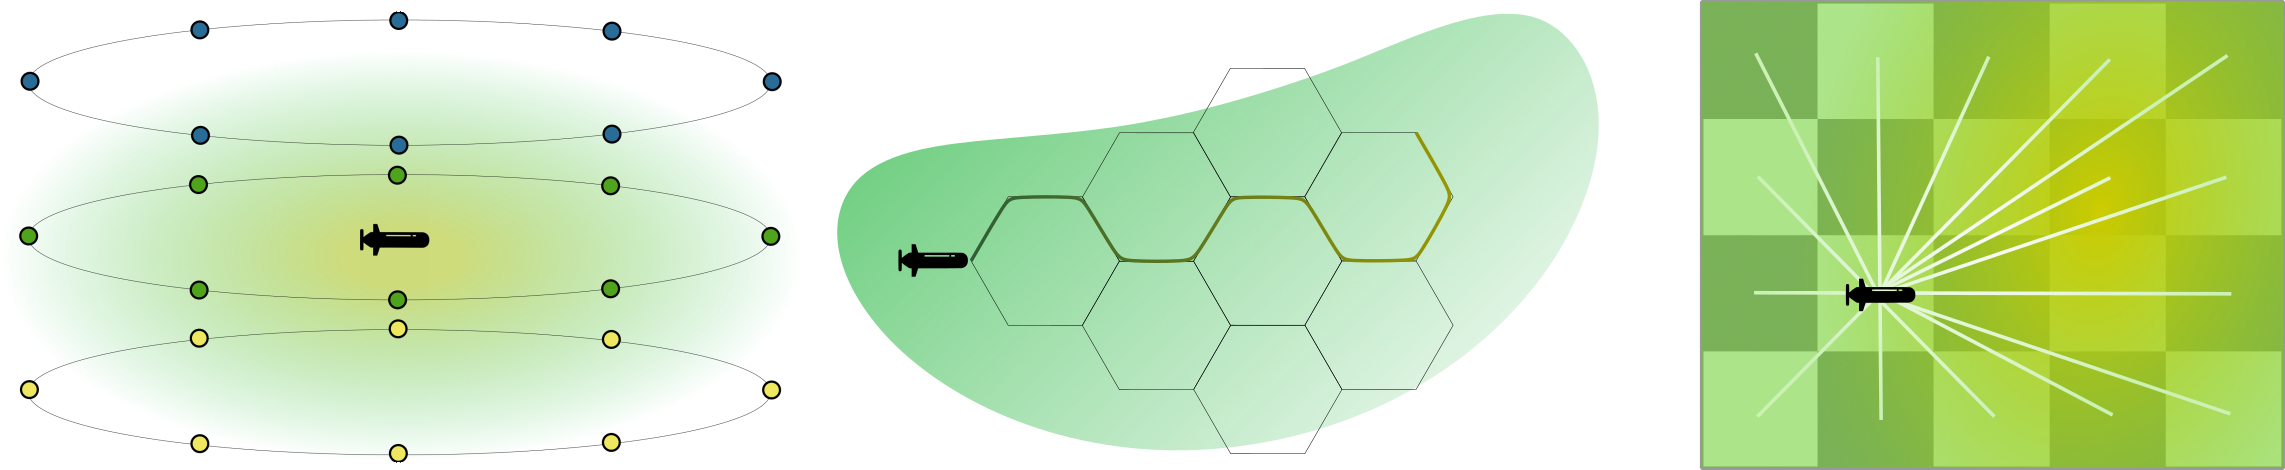
\includegraphics[width= \textwidth]{figures/paths.png}
    \caption{Illustration of planning horizons, from left: myopic, non-myopic, and global.}
    \label{fig:planning}
\end{figure}

\subsection{Waypoints}
In order to apply the utility function on locations in the model, the potential waypoints that make up the path have to be selected, this can be done in several ways. The most common is to have a predefined grid of points in $\mathbb{R}^2$ or $\mathbb{R}^3$, where both measurements are assimilated into and also unobserved locations are estimated for predictive means and variance \cite{kemna2018multi,berget2018adaptive,fossum2019adaptive}This method has proved to be a good baseline, especially in $\mathbb{R}^2$, where computational complexity is constrained. Another approach is to constrain the optimization to fewer dimensions by pre-defining the other path dimensions, as was done in \textcite{fossum2019toward} and \textbf{paper B}, where the adaption was in the depth-domain. One can also generate potential paths from the vehicle kinematic model, where near-term reachability can be a factor, as was done in \cite{stankiewicz2021adaptive}. One promising way of generating potential path is to generate a spatial graph, and use the nodes as potential waypoints, thus connecting several waypoints into a path, this was explored in \cite{fossum2021learning}. 

\subsection{Myopic}
The simplest and most intuitive potential path generation is the \textit{myopic}, or near sighted,  path generation, where the robot looks one step ahead. This method is used in \textbf{paper C \textcolor{red}{todo:maybe yaolin}}, for 3D path generation, where a set of potential waypoints is generated around the vehicle. Creating a ring of potential waypoints has also been suggested\cite{berget2018adaptive,fossum2021learning}, where all potential waypoints have the same distance from the vehicle. This gives the added benefit that the length of the path is irrelevant in the utility function, since all paths are equally long. Depending on the underlying data, model, and utility function, the myopic method might get stuck at local maxima  if the spatial planning horizon is too short. If the distance to the potential waypoints is long, the robot might miss important features that are close by. 

\subsection{Non-myopic}
Expanding from the myopic method, the non-myopic methods\cite{stankiewicz2021adaptive,fossum2021learning} looks further into the space of potential waypoints, at a heightened computational cost (\textbf{papers B, and F \textcolor{red}{todo: yaolin paper ? }}). As the computational cost of evaluating a geometrically expanding tree of potential paths increases with search breadth and depth, it is essential to generate the potential paths intelligently. This can be done by taking the vehicle dynamics into account\cite{stankiewicz2021adaptive}, or by keeping the general direction of the path consistent, as in \textbf{paper B}. However it is generated, the goal of the non-myopic path planning is to escape the pitfalls of the myopic strategies, by not getting stuck at local maxima or miss important features. Further, the non-myopic methods need to be constrained inn computational complexity, such that they are tractable of on-board mission planning.  

\subsection{Global}
The last alternative, available to the gridded methods, is the global path planning \cite{kemna2016adaptive}. In the global methods, all grid points are evaluated as potential waypoints. Depending on the utility function distance penalty, the operator can tune the utility function to the desired behavior. If the grid has a high resolution, this method can be computationally expensive. If, however, the utility function was evaluated along the line towards the waypoint, and normalized for length, one could generate a global and directional set of potential paths, without a distance penalty. 

\section{Utility Functions}
When employing a spatial model of the environment, it can be assessed at points in the domain, both for its predictive mean, but also for its predictive variance, as given in Equations \eqref{eq:mod_gp_pred2} and \eqref{eq:mod_gp_pred3}. These values, along with other features specific to the domain can be used to evaluate different strategies for further sampling, thus these methods are termed \textit{deliberative}; evaluating multiple actions or series of actions. This deliberation often boils down to an optimization over a set of possible options, where the utility function of the optimization is designed for a specific behavior or scientific goal. 


\subsection{Overview}
The practice utilized by \cite{stankiewicz2021adaptive,berget2018adaptive,fossum2018information} is to generate a utility function as a weighted sum of elements relevant to the desired vehicle behavior, the weights need to be carefully selected, and are often selected using simulated data. This can be a challenge, especially if one attempts to use synthetic features, such as gradients. The utility function is evaluated over a possible future sampling locations or sampling paths, in order to find the optimal path. The search can take many forms. \textcolor{red}{expand on the generality of a utility function, link to control law}

\subsection{Predictive mean}
The data driven terms in the utility function often reflect the scientific goal of the adaptive behavior, being designed to draw the robot towards a certain feature. Such features can be maxima, minima or gradients of ocean parameters. In \cite{berget2018adaptive}, higher values of predicted optical backscatter contributed positively in the utility function, whereas \cite{stankiewicz2021adaptive} used the negative value of the predictive dissolved oxygen in order to search for hypoxic (oxygen poor) zones. The spatial gradient of the predictive mean was used in \cite{fossum2019adaptive}, this is not advised from \cite{eidsvik2015value}, as one should use first approximations from the predictive field, rather than to construct features from the field.
\subsection{Uncertainty}
There are several ways of designing an uncertainty reducing utility function, two are described in \cite{fossum2019adaptive}, termed \textit{D-optimality} and \textit{A-optimality}. D-optimality computes the optimal sampling locations by maximizing the reduciton in the determinant of the covariance matrix, as a function of sampling location, or finding the maximum mutual information. This can lead to a more clustered optimal sampling, where as A-optimality can generate a more uniform optimal sampling.  A-optimality evaluates the difference in the trace of the covariance matrix as a function of sampling loaction, and does not take into account the correlation between variables (such as salinity and temperature). These variance reducing strategies were employed in \cite{berget2018adaptive,fossum2018information,stankiewicz2021adaptive} as a prat of the utility function.

\subsection{Entropy}
\subsection{Negative contributions, cost}
In addition to include elements of desire; reduced uncertainty and relevant measurements, there is often a need to limit the utility function by putting a cost on the constraining factors, such as time, distance or battery usage. The euclidean distance from the current location to the sampling location candidate was used as a negative contribution (cost) in the utility function used in \cite{berget2018adaptive}, whereas two model-based approaches for calculating navigation cost are presented in \cite{stankiewicz2021adaptive}. Another cost element that can be used is risk, depending on the robot, the risk can be calculated in many ways; navigational uncertainty, distance from assistance, distance to shipping lanes, remaining battery life, etc.  


\subsection{Mission specific terms}

\subsubsection{Binary Classification}
If the goal is binary classification, e.g. above or below an isotherm, or coral or not coral on a observed patch of seabed, one can employ the Expected Bernoulli Variance, formulated as in Equation (\ref{eq:plan_ebv}), where $P(x)$ is the probability of binary class $x$. 

\begin{align}
    \label{eq:plan_ebv}
    EBV = P(x)(1-P(x))
\end{align}

This will give a high value for regions where $P(x)\approx 0.5$, or where the model is most uncertain in the classification. 



\subsection{Tuning and testing}

\section{Search}

In most of the literature, the evaluation of potential paths or waypoints were described as a simple $argmax$ function, where all potential points were evaluated. This approach can be computationally expensive, especially if evaluating potential paths along a graph. Here one can conduct a myopic search; evaluating only the closest waypoints, a non-myopic search; evaluating several waypoints ahead in a combined fashion, or a global search; evaluating all possible waypoints. In the design of the search, one has to have the computational complexity in mind. A simulation study of methods for search was done by \textcite{fossum2021learning}.
